\documentclass[letterpaper,12pt,oneside]{book}
\usepackage[top=1in, left=1.25in, right=1.25in, bottom=1in]{geometry}
%-----------------------__--------
%https://es.overleaf.com/project/642e50d937469ff17340bdc4
% Tesis UNAM https://tex.stackexchange.com/questions/234265/unam-thesis-title-page-portada-tesis-unam

\usepackage{pdfpages}
\usepackage{lipsum}

\usepackage[T1]{fontenc}
\usepackage[utf8]{inputenc}
\usepackage[spanish,es-nodecimaldot,es-tabla]{babel}
\usepackage{graphicx}
\usepackage{tikz}
\usepackage{setspace}

\title{CARDIAC: La evolución hacia un modelo concurrente y paralelo}

\begin{document}
	\frontmatter
	%\maketitle

    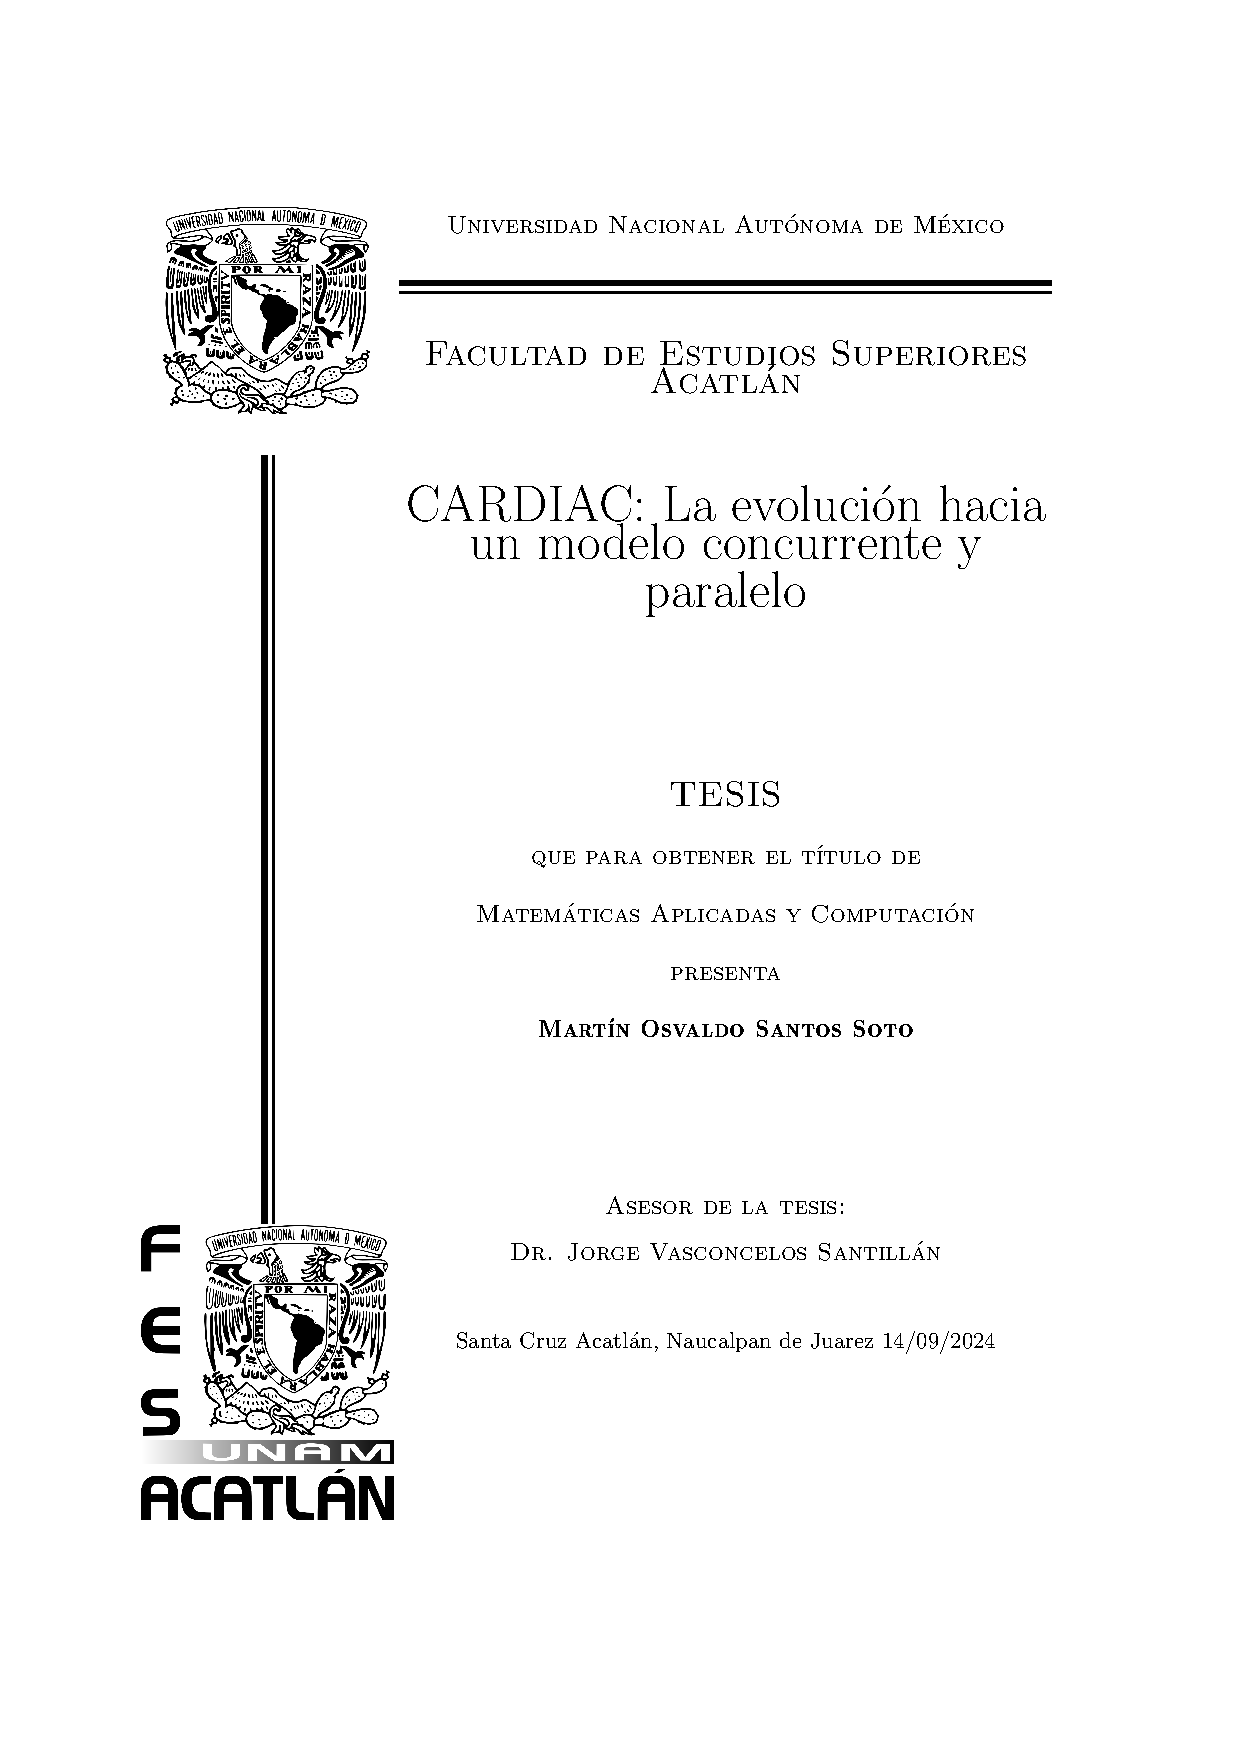
\includepdf{cover.pdf}

%---------------------------------
\chapter*{}
\begin{flushright}%
  \emph{Al club de mis amores, Chelsea ...}
  \thispagestyle{empty}
\end{flushright}

\chapter{Agradecimientos}
%\spacing{1.5}%\doublespacing

\chapter{Abstract}

\chapter{Introducción}


\tableofcontents
\listoffigures

\mainmatter

\chapter{Marco Teórico} %


\section{Inicios de la computación}
   
\section{Historia de las maquinas} 
    \subsection{IBM y Miccrosoft}


\chapter{Metodología}  %
	\section{Necesidad de operaciones concurrentes}
	
	 \section{Evolución hacia el paralelismo}

\chapter{Resultados}  %


\chapter{Conclusiones}

%\bibliographystyle{humannat}
%\bibliography{references}

%\backmatter%@sglvgdor


\end{document}

